\documentclass[12pt]{article}
% Load packages
\usepackage{url}  % Formatting web addresses  
\usepackage{ifthen}  % Conditional 
\usepackage{multicol}   %Columns
\usepackage[utf8]{inputenc} %unicode support
\usepackage{amsmath}
\usepackage{amssymb}
\usepackage{epsfig}
\usepackage{epstopdf}
\usepackage{graphicx}
\usepackage[margin=0.1pt,font=footnotesize,labelfont=bf]{caption}
\usepackage{setspace}
%\usepackage{longtable}
\usepackage{colortbl}
%\usepackage{palatino,lettrine}
%\usepackage{times}
%\usepackage[applemac]{inputenc} %applemac support if unicode package fails
%\usepackage[latin1]{inputenc} %UNIX support if unicode package fails
\usepackage[wide]{sidecap}
%\usepackage[authoryear,round,comma,sort&compress]{natbib}
\usepackage[square,sort,comma,numbers]{natbib}
%\usepackage[authoryear,round]{natbib}
\usepackage{supertabular}
\usepackage{simplemargins}
\usepackage{comment}
\usepackage{lineno}

\urlstyle{rm}

%\textwidth = 6.50 in
%\textheight = 9.5 in
%\oddsidemargin =  0.0 in
%\evensidemargin = 0.0 in
%\topmargin = -0.50 in
%\headheight = 0.0 in
%\headsep = 0.25 in
%\parskip = 0.15in
%\linespread{1.75}
\doublespace

%\usepackage{geometry}
\usepackage{fullpage}

%\bibliographystyle{plain}
\bibliographystyle{plos2009}

\makeatletter
\renewcommand\subsection{\@startsection
	{subsection}{2}{0mm}
	{-0.05in}
	{-0.5\baselineskip}
	{\normalfont\normalsize\bfseries}}
\renewcommand\subsubsection{\@startsection
	{subsubsection}{2}{0mm}
	{-0.05in}
	{-0.5\baselineskip}
	{\normalfont\normalsize\itshape}}
\renewcommand\section{\@startsection
	{subsection}{2}{0mm}
	{-0.2in}
	{0.05\baselineskip}
	{\normalfont\large\bfseries}}	
\renewcommand\paragraph{\@startsection
	{paragraph}{2}{0mm}
	{-0.05in}
	{-0.5\baselineskip}
	{\normalfont\normalsize\itshape}}
\makeatother

%Review style settings
%\newenvironment{bmcformat}{\begin{raggedright}\baselineskip20pt\sloppy\setboolean{publ}{false}}{\end{raggedright}\baselineskip20pt\sloppy}

%Publication style settings

% Single space'd bib -
\setlength\bibsep{0pt}

\renewcommand{\rmdefault}{phv}\renewcommand{\sfdefault}{phv}
\newcommand{\norm}[1]{\left\lVert#1\right\rVert}

% Change the number format in the ref list -
\renewcommand{\bibnumfmt}[1]{#1.}

% Change Figure to Fig.
\renewcommand{\figurename}{Fig.}

% Begin ...
\begin{document}
\begin{titlepage}
{\par\centering\textbf{\Large A novel metaheuristic approach for parameter estimation in high dimensional biochemical networks}}
\vspace{0.05in}
{\par \centering \large{Adithya Sagar, Christine Shoemaker and Jeffrey D. Varner$^{*}$}}
\vspace{0.10in}
{\par \centering \large{School of Chemical and Biomolecular Engineering}}
{\par \centering \large{Cornell University, Ithaca NY 14853}}
\vspace{0.1in}
{\par \centering \textbf{Running Title:}~Parameter estimation in large scale biological systems}
\vspace{0.1in}
{\par \centering \textbf{To be submitted:}~\emph{Biotechnology Journal}}
\vspace{0.5in}
{\par \centering $^{*}$Corresponding author:}
{\par \centering Jeffrey D. Varner,}
{\par \centering Associate Professor, School of Chemical and Biomolecular Engineering,}
{\par \centering 244 Olin Hall, Cornell University, Ithaca NY, 14853} 
{\par \centering Email: jdv27@cornell.edu} 
{\par \centering Phone: (607) 255 - 4258}
{\par \centering Fax: (607) 255 - 9166}
\end{titlepage}
\date{}
\thispagestyle{empty}
\pagebreak
%%%%%%%%%%%%%%%%%%%%%%%%%%%%%%%%%%%%%%%%%%%%%%%%%%%%%%%%%%%%%%%%%%%%%%%%%%%%%%%%%%%%%%%%%%%%%%%%%%%%%%%%%%%
%%%%%%%%%%%%%%%%%%%%%%%%%%%%%%%%%%%%%%%%%%%%%%%%%%%%%%%%%%%%%%%%%%%%%%%%%%%%%%%%%%%%%%%%%%%%%%%%%%%%%%%%%%%
\section*{Abstract}
The problem of parameter estimation presents a significant challenge in the modeling of large complex systems. Mathematical modeling of biological systems is one such area where parameter estimation is a difficult non-linear optimization problem. This problem is further compounded when dealing with parameter vectors of high dimensions. Such problems generally involve expensive function evaluations and it is hard to obtain optimal or near optimal solutions within finite computational time. In this study we present a novel meta-heuristic approach that combines elements of multi-swarm optimization along with dynamically dimensioned search (DDS) to obtain optimal or near optimal solutions of high dimensional biochemical networks within a relatively few function evaluations. We use a multi-swarm optimization technique to generate candidate vectors which are then greedily updated using DDS by dynamically varying the perturbed parameter dimensions. We tested (25 trials with 4000 function evaluations in each trial) this algorithm on a biochemical network of coagulation (148 parameters and 92 species) and compared it's performance against other metaheuristics like Differential Evolution (DE), Particle Swarm Optimization (PSO), Simulated Annealing (SA) and also against DDS alone. The new algorithm outperforms all the other metaheuristics on the coagulation model. The parameter vectors obtained using this approach fit the experimental data well and also make accurate enough predictions on unseen experimental data. We also performed this comparison on commonly used test functions for global optimization and found the same behavior. Further we used two benchmark problems, a genome wide kinetic model with 1759 parameters and a metabolic model of Chinese Hamster Ovary cells with 117 parameters to evaluate the performance of our approach. We  surprisingly outperformed the enhanced scatter search algorithm on these benchmarks and obtained the nominal parameter vector with just 4000 function evaluations. 

{\noindent \textbf{Keywords:}~Parameter identification, Mathematical modeling}

\pagebreak

\setcounter{page}{1}

\linenumbers

\section*{Introduction}

Biological systems interact with one another and with the external world through highly complex biochemical networks. The advent of  \textit {omics} era has provided researchers with a deluge of data about these networks. Over the last decade, with an increase in computational power, large scale mathematical modeling of biological systems has evolved as a powerful paradigm to understand this data deluge and to effectively characterize these complex biochemical interactions.  

The development of such mathematical models for biochemical networks can be broadly decomposed into two tasks a) Model construction b) Model calibration or Parameter Estimation. Model construction involves translating existing knowledge about the network (i.e. entities in the network, interactions amongst the entities, types of interactions) along with reasonable assumptions into an appropriate mathematical 
framework.  Some popular mathematical formulations have been Ordinary Differential Equations (ODEs), Boolean and fuzzy logic, probabilistic graphical models etc. [REFHERE]

Model calibration or parameter estimation follows the model construction step.  In this step the model is trained against experimental data to determine the model parameters that give a good fit against experimental data. Model simulation using these parameters is then done and the results are validated using hitherto unseen experimental data. If validation leads to unsatisfactory results model construction and calibration are repeated iteratively till we get satisfactory results. 

With the capacity to construct or formulate very large biological models, more often than not, parameter estimation has become the bottleneck in large scale mathematical modeling of biological systems. The problem of parameter estimation if generally framed as a non-linear optimization problem.


\textit  {\Large Equation needs to be written and explained terms}

\begin{eqnarray}
	\mathcal{G}_{new}(\mathbf{J})& = &\mathcal{G}(\mathbf{J})+\mathbf{r}_{normal}(\mathbf{J})\sigma(\mathbf{J})
\end{eqnarray}

The objective function from equation ---  is minimized using appropriate optimization technique to estimate the model parameters. Due to the complex dynamics of biological systems these problems are multi-modal i.e. most of them have multiple local minima or maxima. The non-linearity of the problem coupled with multi-modality is a substantial challenge and generally renders the local optimization techniques incapable of obtaining an optimal solution.   
\textit {In many of these problems derivative information is absent or the objective function may be discontinuous. This hinders the use of deterministic optimization techniques that require the problem to be convex and other derivative/gradient based optimization methods. Most of these methods are computationally expensive and for optimization of large-scale systems, this becomes prohibitively expensive.  Heuristic approaches have been promising in this regard, however most of the population-based heuristics take a large number of function evaluations and have computationally complex operations, which reduces their effectiveness in finding feasible solutions with limited computational resources and time. Hybrid methods that couple heuristics with derivative based methods}

The problem get further compounded when we have parameter vectors of very high dimensions. In this study we developed a novel meta heuristic approach that combines multi-swarm particle swarm optimization with dynamically dimensioned search (DDS)to obtain optimal or near optimal solutions to high-dimensional, non-linear biological models within a relatively few function evaluations.

A bit of history on DDS
Why coagulation model? feed back loops, parameter identifiability, tight regulation and also high dimensional


\subsection *{Parameter Estimation Literature}

\subsection *{Modeling methodologies Literature} 
 Shuler and co-workers constructed large-scale dynamic metabolic models of E.coli that were based ordinary differential equations (ODEs). Various aspects of E.colis cellular processes like RNA synthesis, chromosome synthesis, cellular energy expenditure etc. were modeled using coupled non-linear ordinary differential equations. Post genomic era saw the rise of flux balance analysis (FBA), a static, constraint based modeling approach for microbial metabolism. FBA assumes a pseudo steady-state and reduces genome-scale kinetic models to a set of static mass balances. These mass balances are represented using an underdetermined set of linear algebraic equations. The advantage is such a system of equations can be solved efficiently for very large systems. 

The dynamics of signal transduction systems are commonly modeled using ODEs [Refs]-----. One of the advantages of using ODEs is that the dynamics of large-scale systems can be described with a great degree of mechanistic detail. Over the last half a decade we have seen the construction of increasingly large-scale ODE models of signal transduction systems. Chen et al. built a mass action model of ErbB signaling pathways with 499 ODEs and 229 parameters. Tasseff et al analyzed retinoic acid induced differentiation of uncommitted precursor cells using a dynamic ODE model with 729 proteins and protein complexes interconnected with 1356 interconnections. Luan et al captured the key aspects of coagulation using an ODE model with 193 proteins and protein complexes with 301 kinetic parameters.  

  Boolean logic, probabilistic modeling and fuzzy logic are other mathematical frameworks that are used for mechanistic modeling of signal transduction systems. Choi et al modeled the p53 signaling network that affects cellular response to DNA damage using Boolean logic. ------.  In Boolean modeling of signal transduction systems the network entities i.e. proteins assume a value of 0 or 1 based on their activation levels. Fuzzy logic models offer a greater detail by allowing protein activation to take on a range of discrete values between 0 and 1. Mitsos et al. used the constrained fuzzy logic approach (cFL) wherein protein activation takes real values and a transfer function (TF) is used to propagate the signal along the network. Boolean and fuzzy logic models offer a relatively simpler mathematical formulation as compared to ODE models and are not encumbered with a large number of parameters. However these models are static in nature and offer a more qualitative view of the system. In addition to these deterministic formulations, stochastic modeling is another way of representing biochemical networks. Stochastic models are primarily based on stochastic differential equations also called Langevin equations to describe the dynamics of biochemical network ----- [Refs]. Stochastic models are limited to describing dynamics of small-scale biochemical networks and are computationally very expensive to characterize even in very small biological systems. 

 \clearpage

\section*{Results}
\subsection{Coagulation model formulation}

Coagulation is an archetype biochemical network that is highly interconnected and tightly regulated with multiple positive and negative feedback loops. The biochemistry underlying coagulation, though quite complex has been well studied [REFHERE], and reliable experimental coagulation models have been developed [REFHERE]. This makes it an ideal system for mathematical modeling and parameter estimation. Coagulation is regulated by a set of serine proteases also known as coagulation factors and blood platelets. The coagulation factors are generally in an inactive state and are known as zymogens. These zymogens are activated through certain triggers. These trigger events like injury or trauma or sepsis expose factors like collagen, tissue factor and von Willebrand factor (vWF) to blood. The exposure of these factors to blood kick-starts a series of convergent cascades that lead to conversion of zymogen prothrombinase to thrombin.   Luan et al. modeled coagulation using coupled non-linear ordinary differential equations with 148 reactions and 92 species [REFHERE]. The model was validated using 21 published datasets. The model parameters used in the simulation were drawn from various literature sources. 

We compared the performance of DDSMLSPSO on this model of coagulation against commonly used meta heuristics like Simulated Annealing (SA), Differential Evolution (DE), Particle Swarm Optimization (PSO) and also against DDS. To train the model parameters we used data sets from TF-VIIa initiated coagulation with no anticoagulants. The objective error function is a linear combination of two different error functions that used data sets representing coagulation initiated with different concentrations of TF-VIIa (5pm, 5nm).  Since this is an expensive error function we restricted the number of function evaluations to 4000 for each algorithm. We performed 25 trials of this experiment. DDSMLSPSO exhibits a much faster rate of error convergence and has a much lower final error as compared to the other algorithms (Figure 3). Within the first 1000 function evaluations (swarm phase) of DDSMLSPSO there is a very rapid drop in error. Subsequently, again after 2500 function evaluations (dynamically dimensioned phase) the error drops quickly. Overall at the end of 4000 function evaluations DDSMLSPSO minimizes the error to much a greater extent than any of the other algorithms. Amongst the rest of the algorithms DDS and SA have a faster rate of drop in error as compared to PSO or DE. However after 1500 function evaluations, the objective error remains nearly constant.  

Figure 2 shows the fit between model predictions and experimental data. The solid lines represent the mean value of prediction over 25 trials and the shaded region represents the 99\% confidence interval.  Figure 3 shows model predictions on completely 'unseen'  or untrained data sets where coagulation was initiated with 500pm, 50pm, 10pm concentrations of TF-VIIa respectively.  The parameters that were obtained by simultaneous training on the 2 data sets were able to 'fit' the experimental data well within a few number of function evaluations. 

\subsection*{Performance on Benchmark functions}

We compared the performance of these algorithms on commonly used test functions for global optimization. Figure-xxx shows the rate of error convergence on a 300D rastrigin function where DDSMLSPSO clearly outperforms the other approaches. In Figure-yyyy, on a 300D ackley function we see the same trend wherein  DDSMLSPSO reaches the minimum much faster than other algorithms.

Villaverde and co-workers recently published a set of benchmark problems to evaluate parameter estimation methods [REFHERE]. From a computational cost perspective problems they categorized the problems as most expensive, intermediate and least expensive. We evaluated the performance of our algorithms on a problem from the most expensive and least expensive categories. Table 1 shows that 

\begin{table}[h!]
\centering
\begin{tabular}{|c c c c c c c|} 
 \hline
 ModelID & Coagulation & B1 & B4 & Ackley300D & Rastrigin300D&\\ [0.5ex] 
 \hline
 Upper bound&$1000.pnom$& ${5.pnom}$ & ${5.pnom}$ &${30}$ &$5.12$& \\  [0.5ex]
 Lower bound&$0.001.pnom$& ${0.2.pnom}$ & ${0.2.pnom}$&${-15}$&$-5.12$&\\ [0.5ex]
 CPU time &$5.6$ ${hours}$ &$38.308$ ${hours}$ & $6.2$ ${minutes}$& ${2.8}$${seconds}$&${2.6}$${seconds}$& \\ [0.5ex]
 Function Evaluations &$4000$&$4000$&$4000$&$4000$&$4000$&\\ [0.5ex]
 Initial Objective Value & $1.0589.10 ^{10}$ & $1.4275.10 ^{7}$ &$1.8536.10 ^{7}$&$21.12$&$99.985$&\\ [0.5ex] 
 Final Objective Value & $2.9223.10^{3}$ & $4.96.10^{5}$ & $38.9375$&$0$&$0$&\\ [0.5ex]
 Nominal Objective Value & $4.7785�10^{6}$& $1.0986�10^{6}$ & $39.0676$&$0$&$0$&\\ [1ex]
 \hline
\end{tabular}
\caption{Table with optimization settings and results for coagulation and different benchmarks using DDSMLSPSO.}
\label{table:1}
\end{table}



\clearpage
\section*{Discussion}
\clearpage
\section*{Materials and Methods}
\subsection*{Formulation and solution of coagulation model equations.}
\subsection*{Optimization Strategy}
Dynamically dimensioned multi-swarm particle swarm optimization (DDSMLSPSO) is a novel optimization approach that combines elements from multi-swarm based PSO methods  with DDS. The goal of this approach is to obtain optimal or near optimal parameters for high-dimensional complex biological systems within a pre-specified number of function evaluations. 

Using Latin Hyper Squares we randomly initialized a swarm of $\mathcal{K}$-dimensional particles (represented as ${x}_{i}$), wherein each of these particles corresponds to an $\mathcal{K}$-dimensional parameter vector. After initialization, the particles were grouped into different sub-swarms randomly. Thereafter within each sub-swarm ${S}_{k}$,  particles were updated according to the following rule.
\begin{eqnarray}
	\mathbf{x}_{i,j} &=&\theta_{1,j-1}\mathbf{x}_{i,j-1} + \theta_{2}\mathbf{r}_{1}\left(\mathcal{L}_{i} - \mathbf{x}_{i,j-1}\right) + \theta_{3}\mathbf{r}_{2}\left(\mathcal{GL}_{k} - \mathbf{x}_{i,j-1}\right) 
\end{eqnarray}

where $\left(\theta_{1},\theta_{2},\theta_{3}\right)$ are adjustable parameters, $\mathcal{L}_{i}$ denotes the best local solution found by particle $i$ till function evaluation $j$-$1$, and
$\mathcal{GL}_{k}$ denotes the best local solution found over the population of all particles within the swarm ${S}_{k}$. The quantities $r_{1}$ and $r_{2}$ denote uniform random vectors with the same dimension as the number of unknown model
parameters ($\mathcal{K}\times{1}$). In our algorithm the parameter $\theta_{1,j-1}$ depends on the function evaluations and is controlled according to the following equation

\begin{eqnarray}
	\mathbf \theta_{1,j}&=&((\mathbf{N}-{j})*(\mathbf{w}_{max}-\mathbf{w}_{min}))/(\mathbf{N}-{1}) + \mathbf{w}_{min}
\end{eqnarray}

where $\mathbf{N}$ represents the total number of function evaluations, $\mathbf{w}_{max}$ and $\mathbf{w}_{min}$ are the maximum and minimum inertia weights respectively. While updating the particle, we made sure all dimensions of the solution represented by the particle was within bounds using a reflection boundary condition. After every $\mathbf{g}$  function evaluations, the particles within all sub-swarms were mixed and then randomly redistributed to a new sub-swarm. The particles were then again updated according Eq.1. This process continued till $\mathcal{FR}*\mathbf{N}$ number of functions evaluations, where $\mathcal{FR}$ represents the fraction of evaluations with the multi-swarms. At the end of these function evaluations, we froze all the solutions represented by various particles and chose the particle with best solution among $\mathcal{GL}_{1} \cdots \mathcal{GL}_{NS}$ as the initial candidate vector $\mathcal{G}$ for the remaining $({1}-\mathcal{FR})*\mathbf{N}$ number of function evaluations.   

This particle was then updated according to the following rule 

\begin{eqnarray}
	\mathcal{G}_{new}(\mathbf{J})& = &\mathcal{G}(\mathbf{J})+\mathbf{r}_{normal}(\mathbf{J})\sigma(\mathbf{J})
\end{eqnarray}

where $\mathbf{J}$ represents the a vector containing the specific dimensions being perturbed, ${r}_{normal}$ denotes a normal random vector of the same dimensions as $\mathcal{G}$. $\sigma$ is the amplitude of perturbation given by following equation

\begin{eqnarray}
	\sigma& = &\mathbf{R}(\mathcal{MAX} -\mathcal{MIN})
\end{eqnarray}

where $\mathbf{R}$ is the scalar perturbation size parameter, $\mathcal{MAX}$ and $\mathcal{MIN}$ are ($\mathcal{K}\times{1}$) vectors that represent the maximum and minimum bounds on each dimension. The probability $\mathcal{P}$ that a specific dimension is perturbed is a  monotonically decreasing function that decreases with the number of function evaluations. $\mathcal{P}$ can be any monotonically decreasing function, in our approach we used the following function
\begin{eqnarray}
	\mathcal{P}_{j}&=&{1}-\log(j/ (\beta({1}-\mathcal{FR})*\mathbf{N}))
\end{eqnarray}

where $\beta$ is the perturbation frequency probability modulator. Thus the number of dimensions of the candidate vector that are updated or perturbed decreases with the as the number of function evaluations increase. These updates are greedy in nature that is $\mathcal{G}_{new}$ becomes the new solution vector only if it is better than the old one $\mathcal{G}$.  


\begin{figure}[H]
\centering
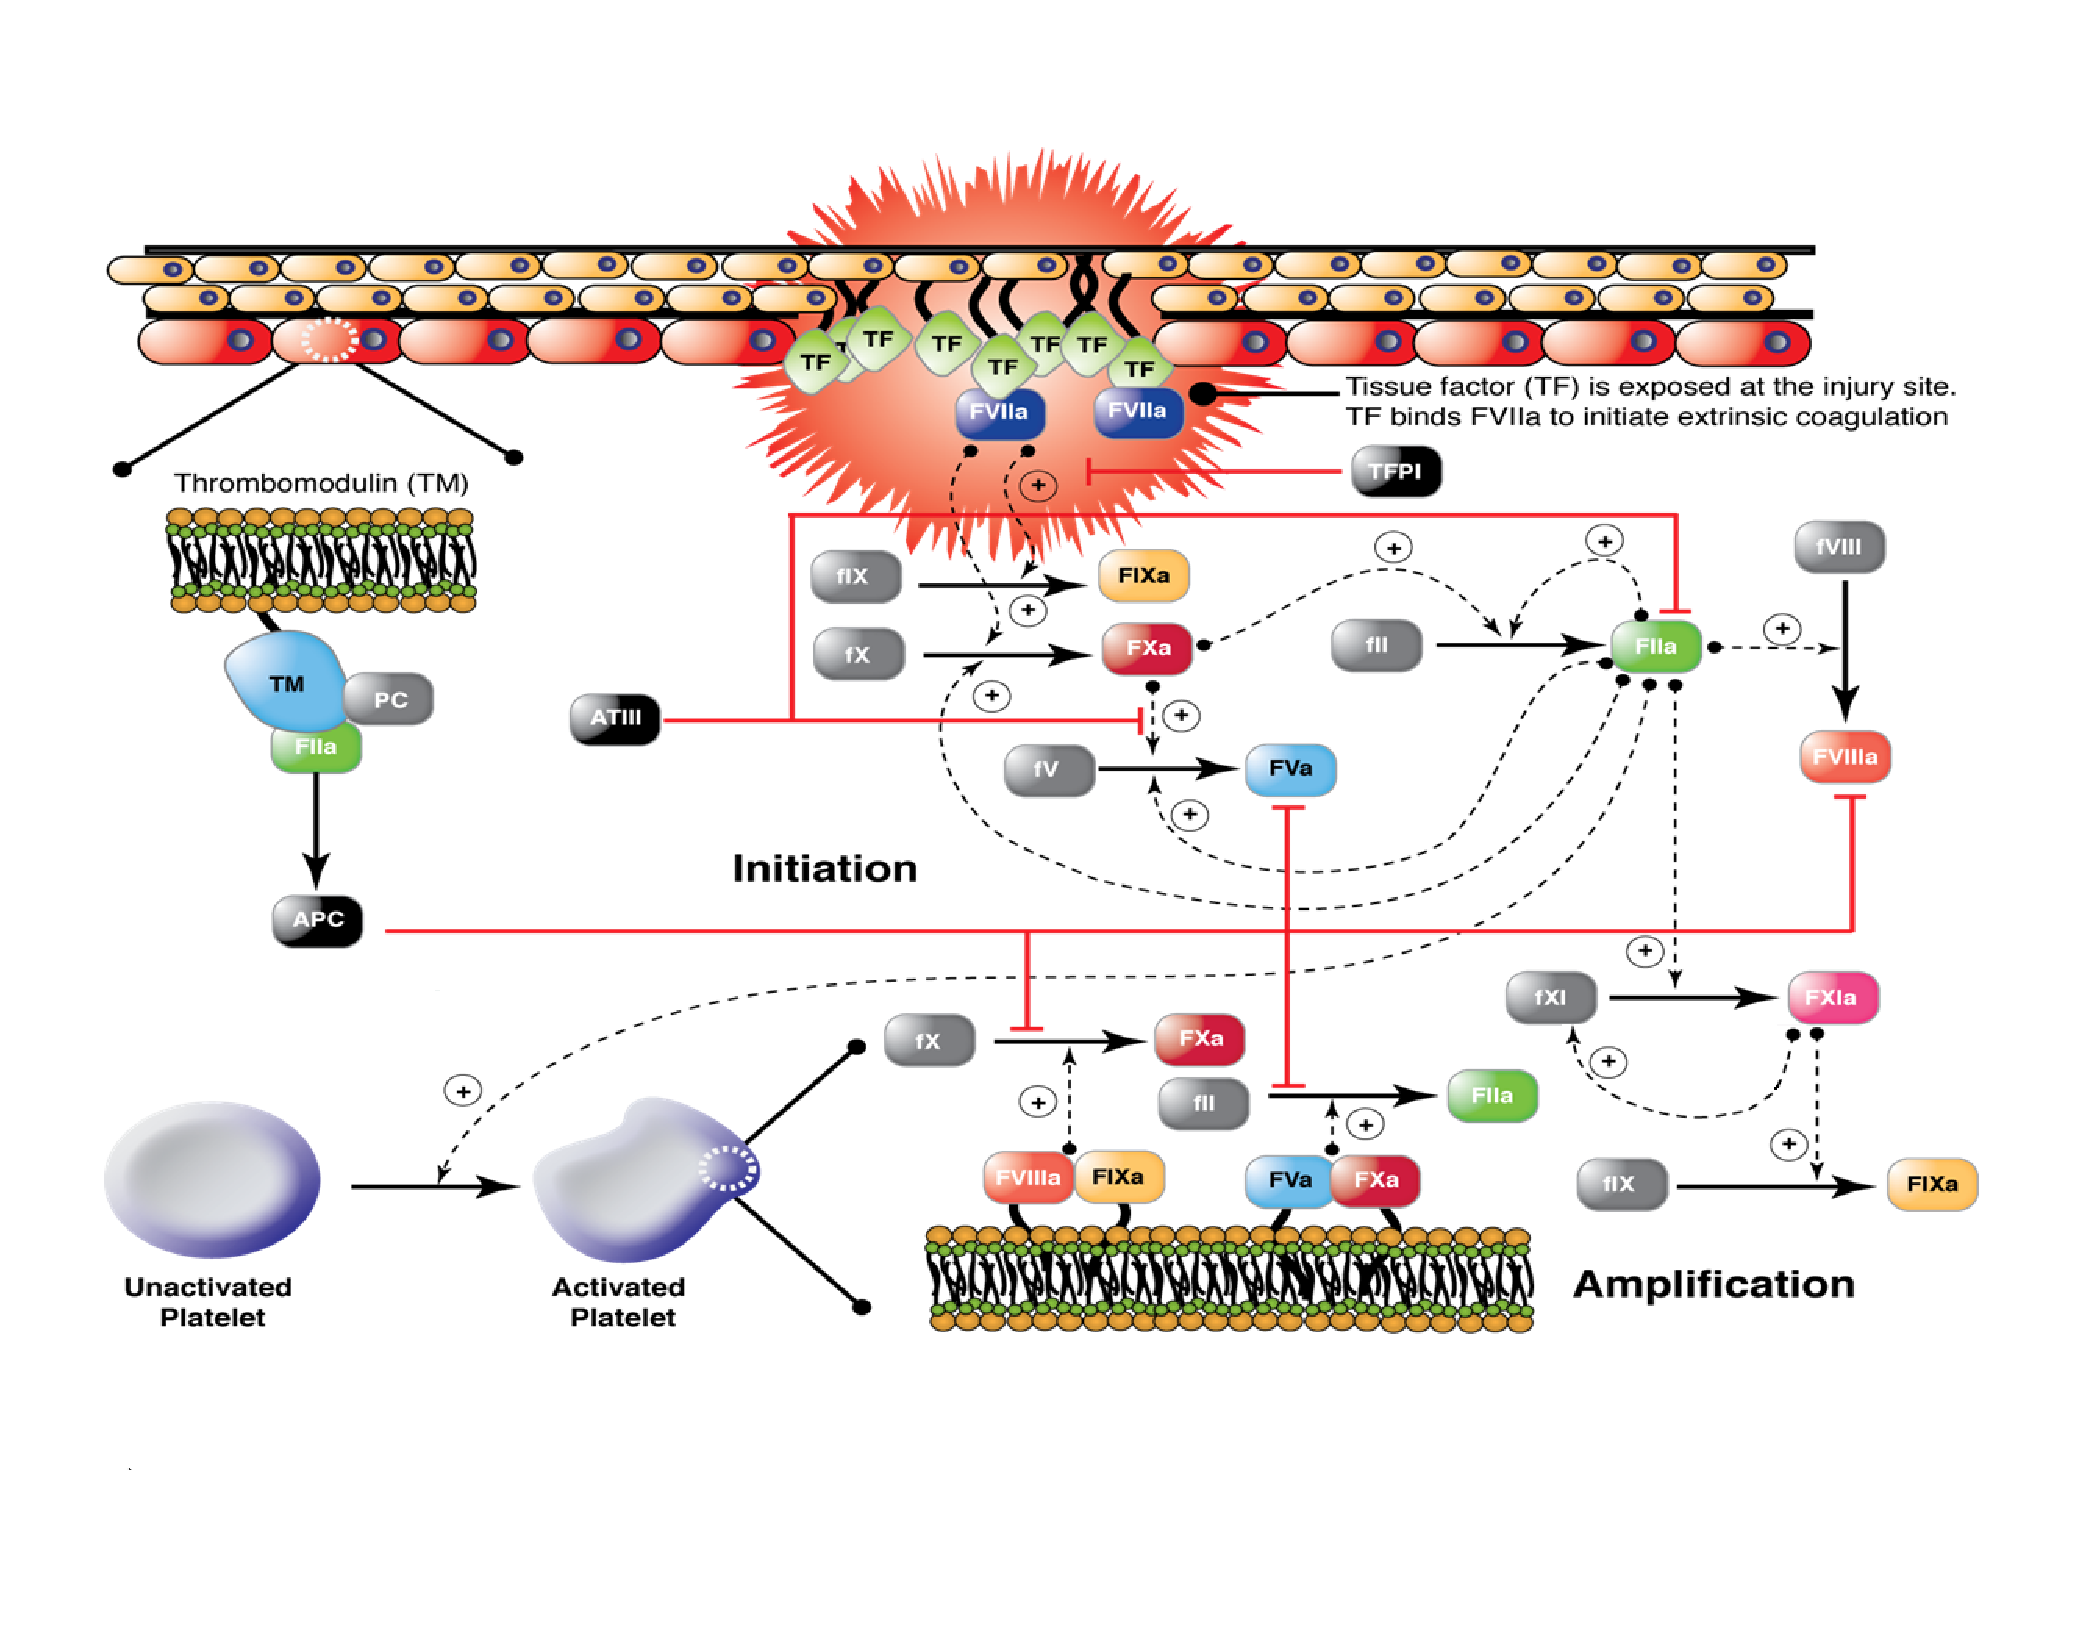
\includegraphics[width=1.00\textwidth,height=0.7\textheight]{./figs/Figure_2_CoagulationNetwork.pdf}
\caption{Schematic of the extrinsic and intrinsic coagulation cascade.Upstream coagulation factors are activated by materials exposed following vessel injury chief among these tissue factor (TF) [Ref] Tissue factor and activated factor VIIa (FVIIa) form a complex that activates factor X (fX) and IX (fIX). FXa activates downstream factors including factor VIII (fVIII) and fIX. Factor V (fV) is primarily activated by thrombin (FIIa). In addition, we included a secondary fV activation route involving FXa. FXa and FVa form a complex (prothrombinase) on activated platelets that converts
prothrombin (fII) to FIIa. FIXa and FVIIIa can also form a complex (tenase) on activated platelets which catalyzes FXa formation. Localized
platelets are activated by external signals such as adenosine diphosphate (ADP) and thromboxane A2 (TXA2) or thrombin through
protease-activated receptors (PARs)[Ref] Thrombin also activates upstream coagulation factors, forming a strong positive feedback ensuring
rapid activation. Tissue factor pathway inhibitor (TFPI) downregulates FXa formation and activity by sequestering free FXa and TF-FVIIa in a
FXa-dependent manner. Antithrombin III (ATIII) neutralizes all proteases, making it perhaps the most powerful control element in the cascade.
Thrombin itself plays an inadvertent role in its own inhibition by binding the surface protein thrombomodulin (TM), expressed on normal
vasculature[Ref] The IIa-TM complex catalyzes the conversion of protein C (PC) to activated protein C (APC), which attenuates the coagulation response by the proteolytic cleavage of fV/FVa and fVIII/FVIIIa [Ref] }\label{fig-flux-pattern}
\end{figure}


\begin{figure}[H]
\centering
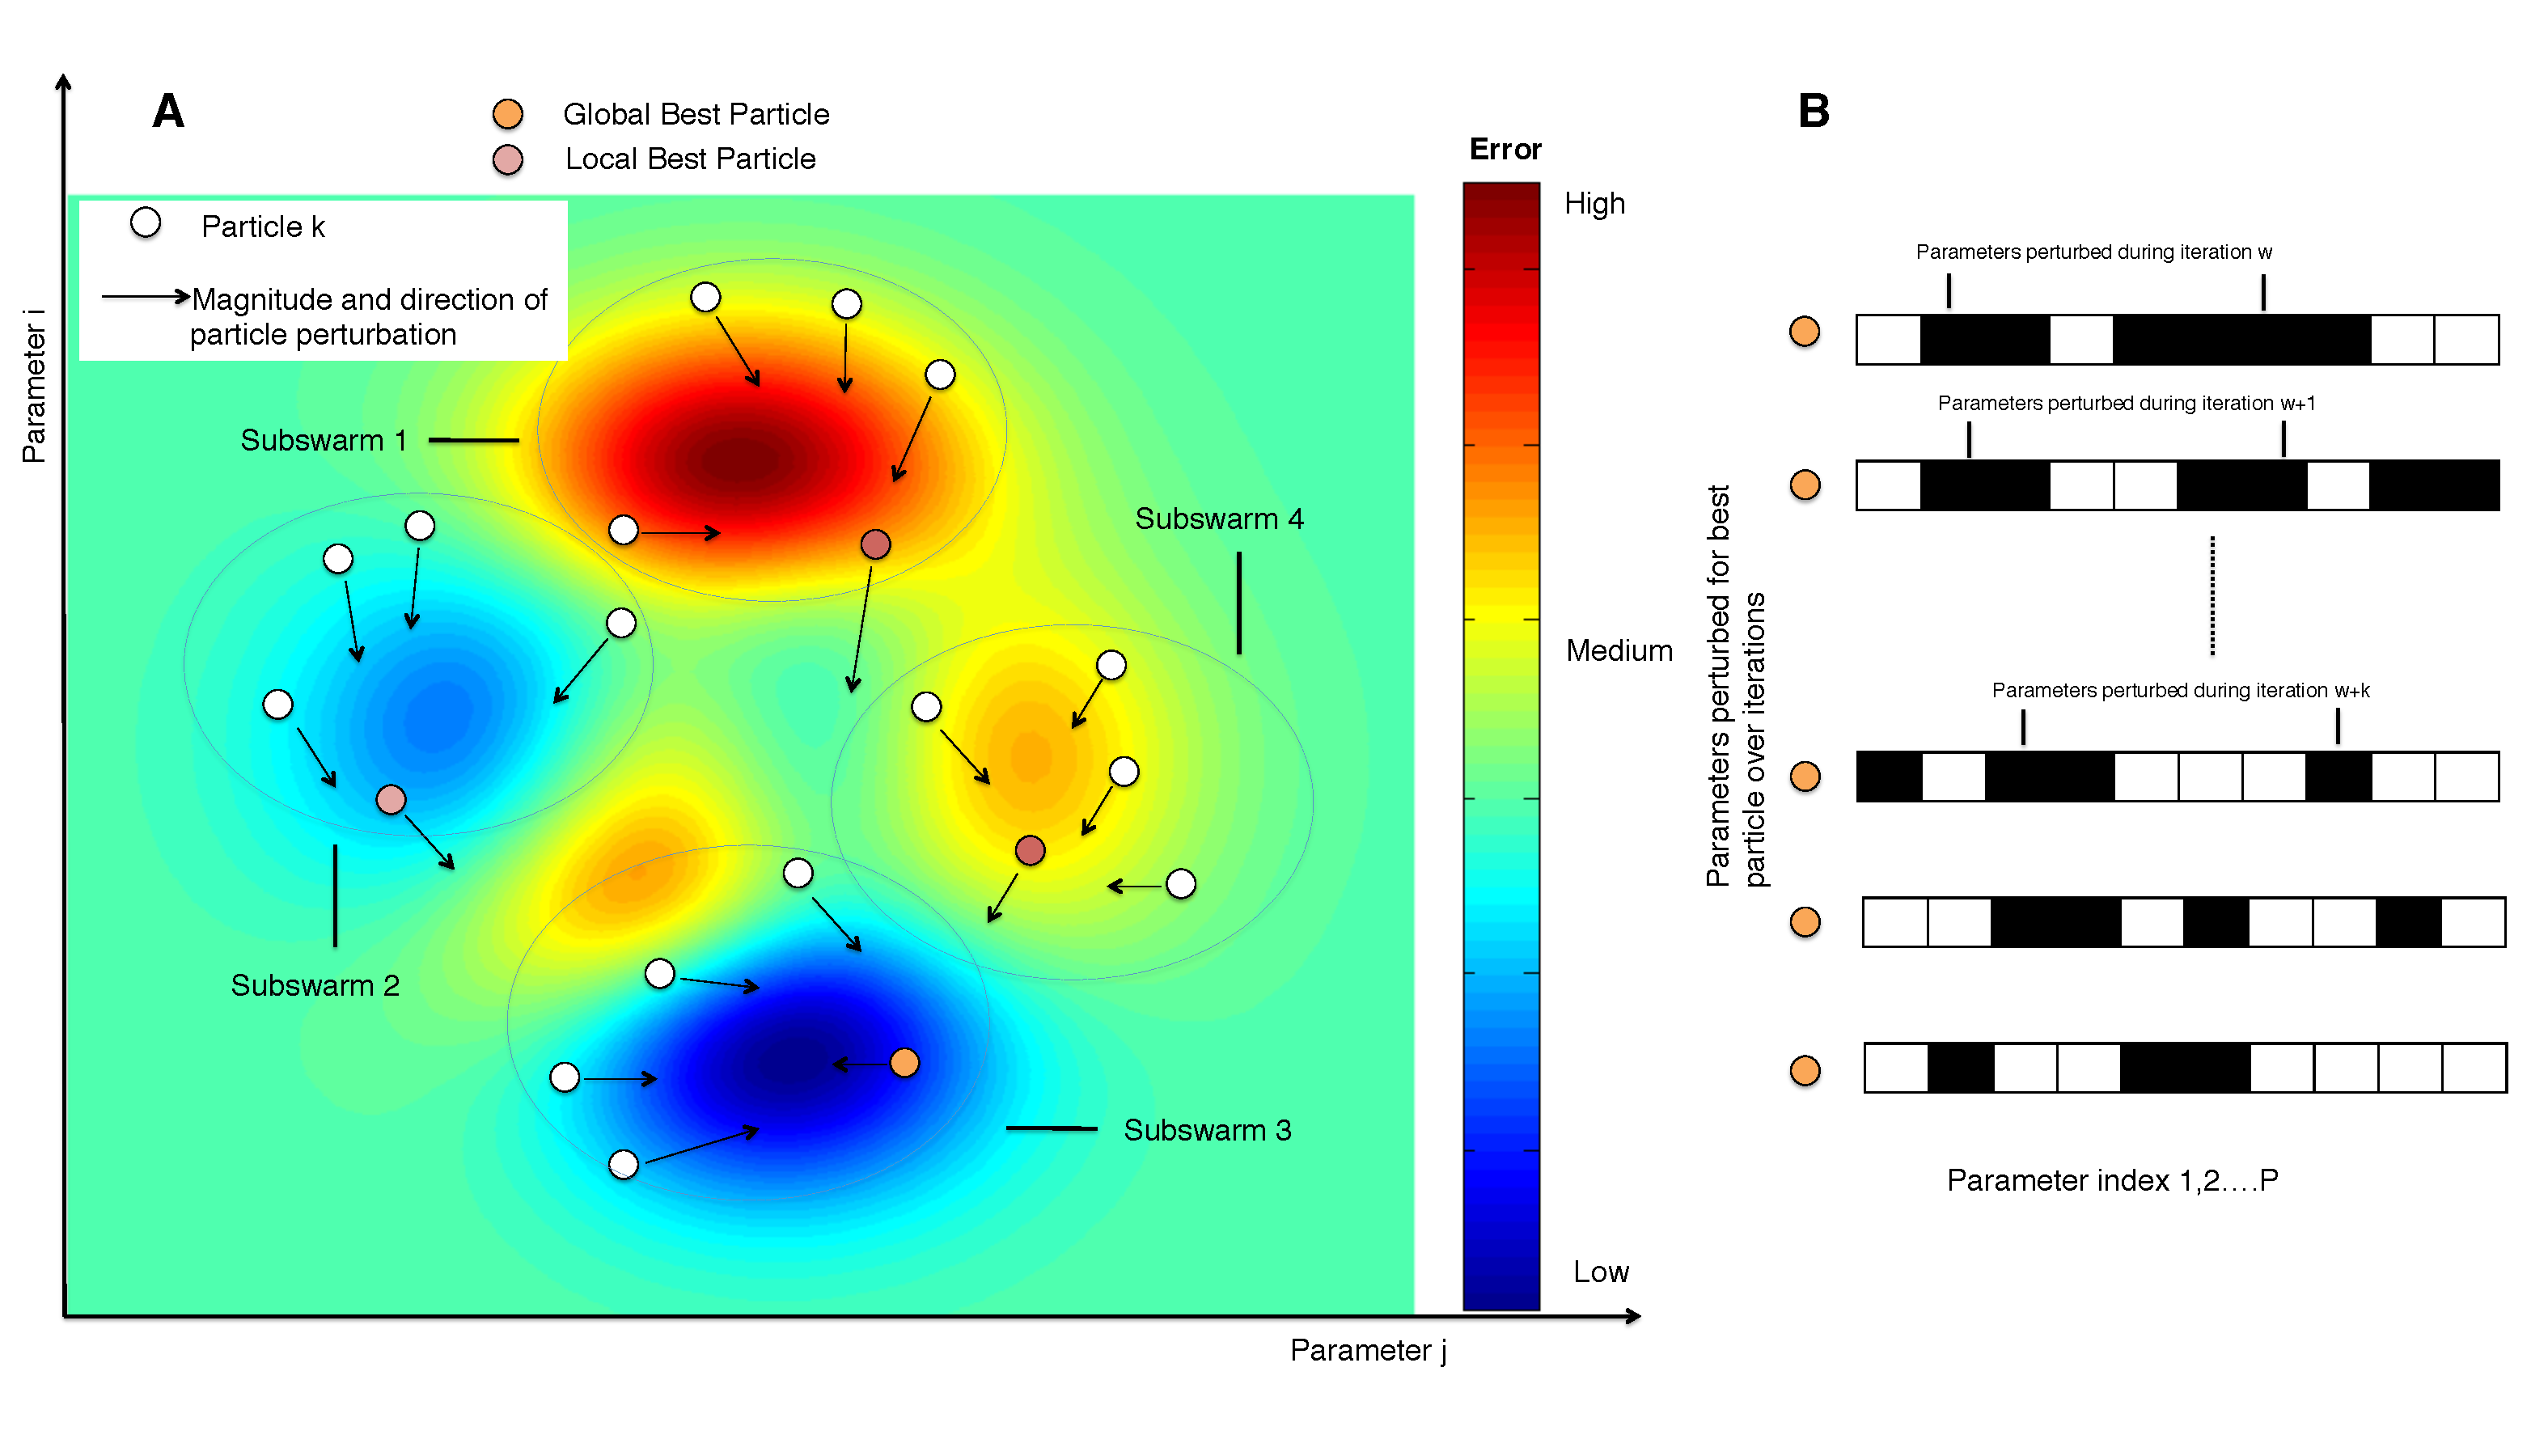
\includegraphics[width=1.0\textwidth,height=0.5\textheight]{./figs/Figure_1_Algorithm.pdf}
\caption{Multi Swarm Particle Swarm Optimization with Dynamically Dimensioned Search. \textbf{A}: Each particle represents an N dimensional parameter vector. Particles are randomly initialized and grouped into various sub-swarms. The magnitude and direction of the movement a particle is influenced by the position of the best particle in its swarm and also by its own experience. After a certain number of function evaluations the particles are mixed and randomly assigned to different swarms. At the end of the evaluations assigned to swarm search, the global best particle amongst all sub-swarms is chosen as the candidate parameter vector for Dynamically Dimensioned Search \textbf{B}: The candidate vector does a greedy search in a dynamic neighborhood. This done by dynamically adjusting the number of parameter dimensions that are perturbed in each evaluation step. The number of dimensions that are perturbed generally decreases as the number of iterations increase. This preserves the optimality of the solution as the number of evaluations increases. 
}\label{fig-algorithm}
\end{figure}

\begin{figure}[H]
\centering
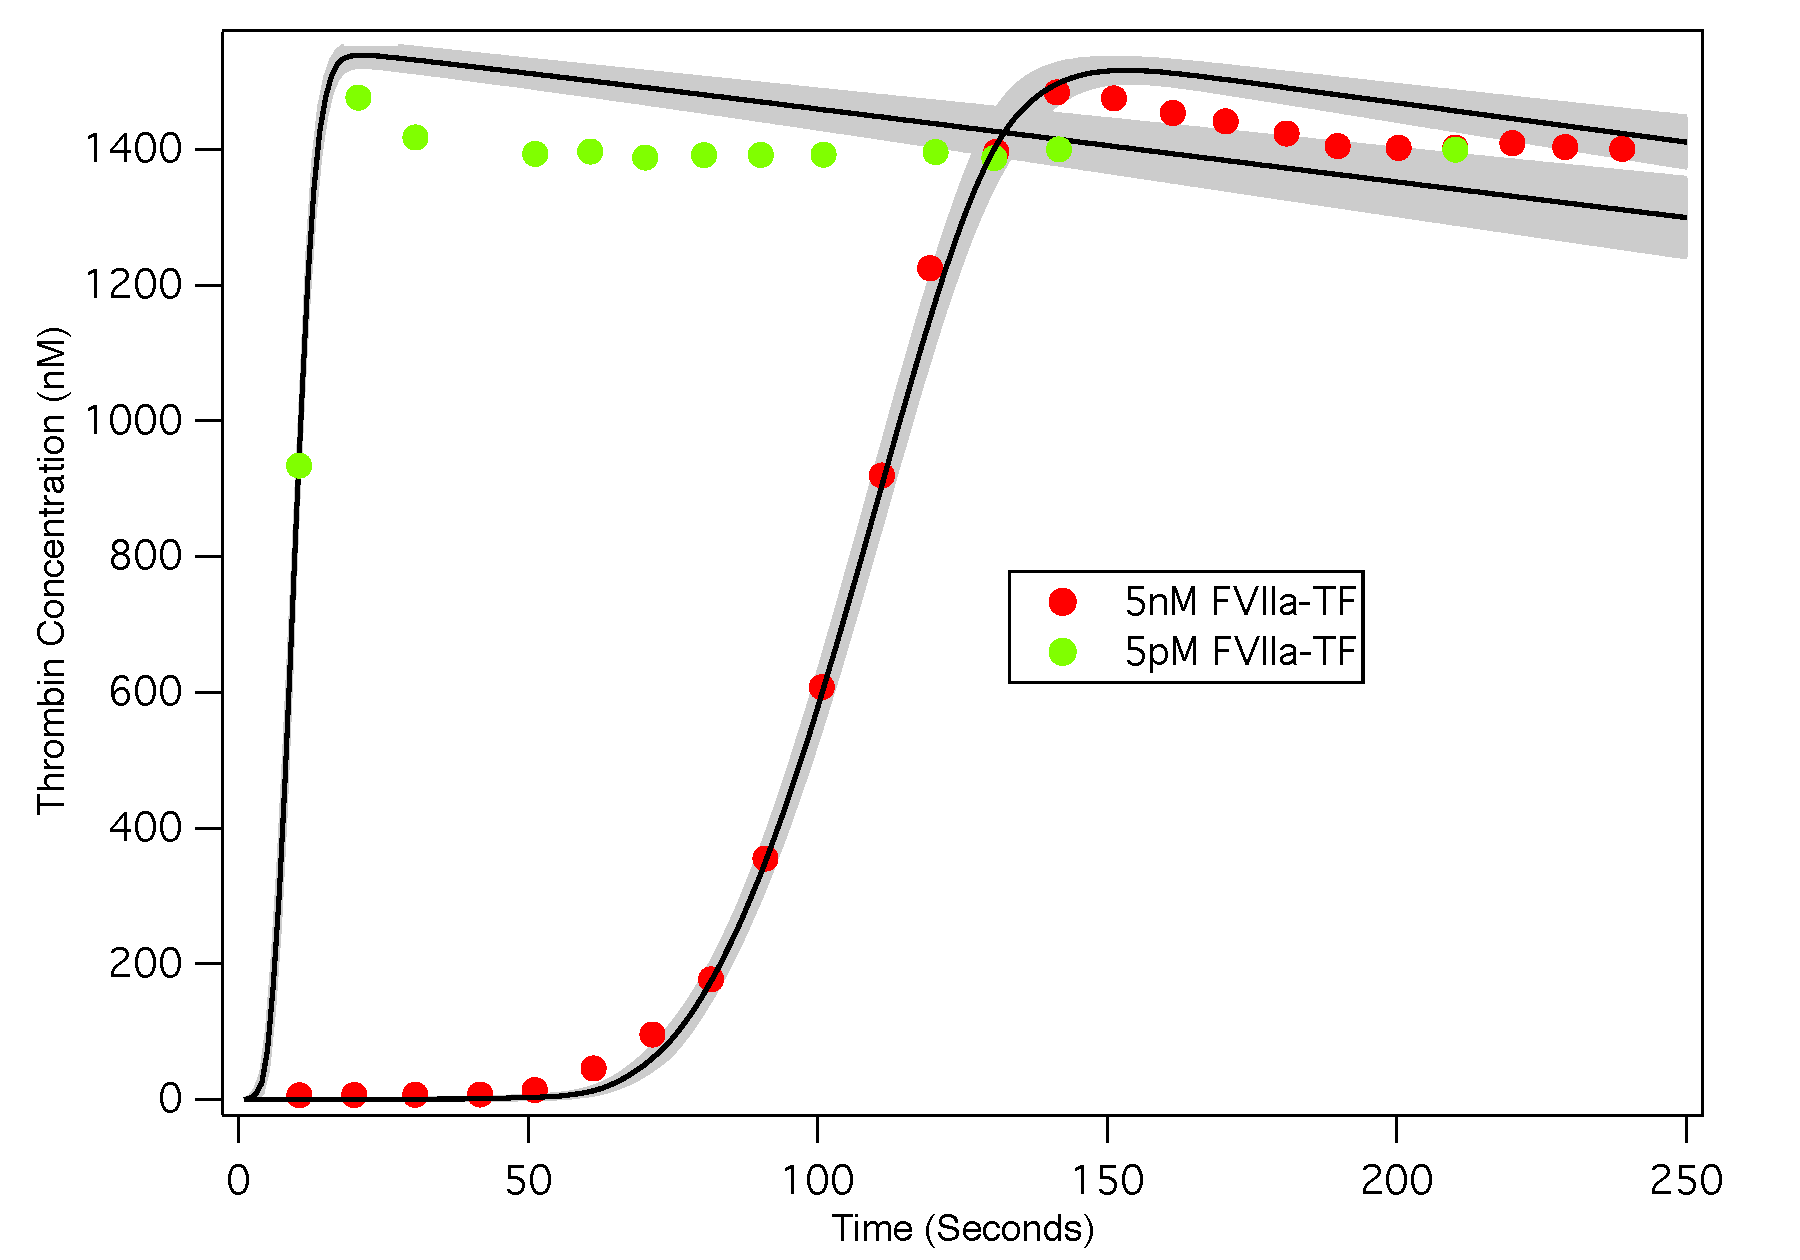
\includegraphics[width=1.0\textwidth,height=0.5\textheight]{./figs/Figure_4_Sim_Train_E1_E5.pdf}
\caption{Model fits on experimental data using DDSMLSPSO. The model parameters were estimated using DDSMLSPSO. Solid black lines indicate the simulated mean thrombin concentration using parameter vectors from $N$= 25 trials. The grey shaded region represents the 99\% confidence estimate of the mean simulated thrombin concentration. The experimental data is reproduced from the synthetic plasma assays of Mann and co-workers [REFHERE]. Thrombin generation is initiated by adding Factor VIIa-TF (5nM - Red and 5pM - Green) to synthetic plasma containing 200 $\mu$mol/L of phospholipid vesicles (PCPS) and a mixture of coagulation factors (II,V,VII,VIII,IX,X and XI) at their mean plasma concentrations.
}\label{fig-train}
\end{figure}


\begin{figure}[H]
\centering
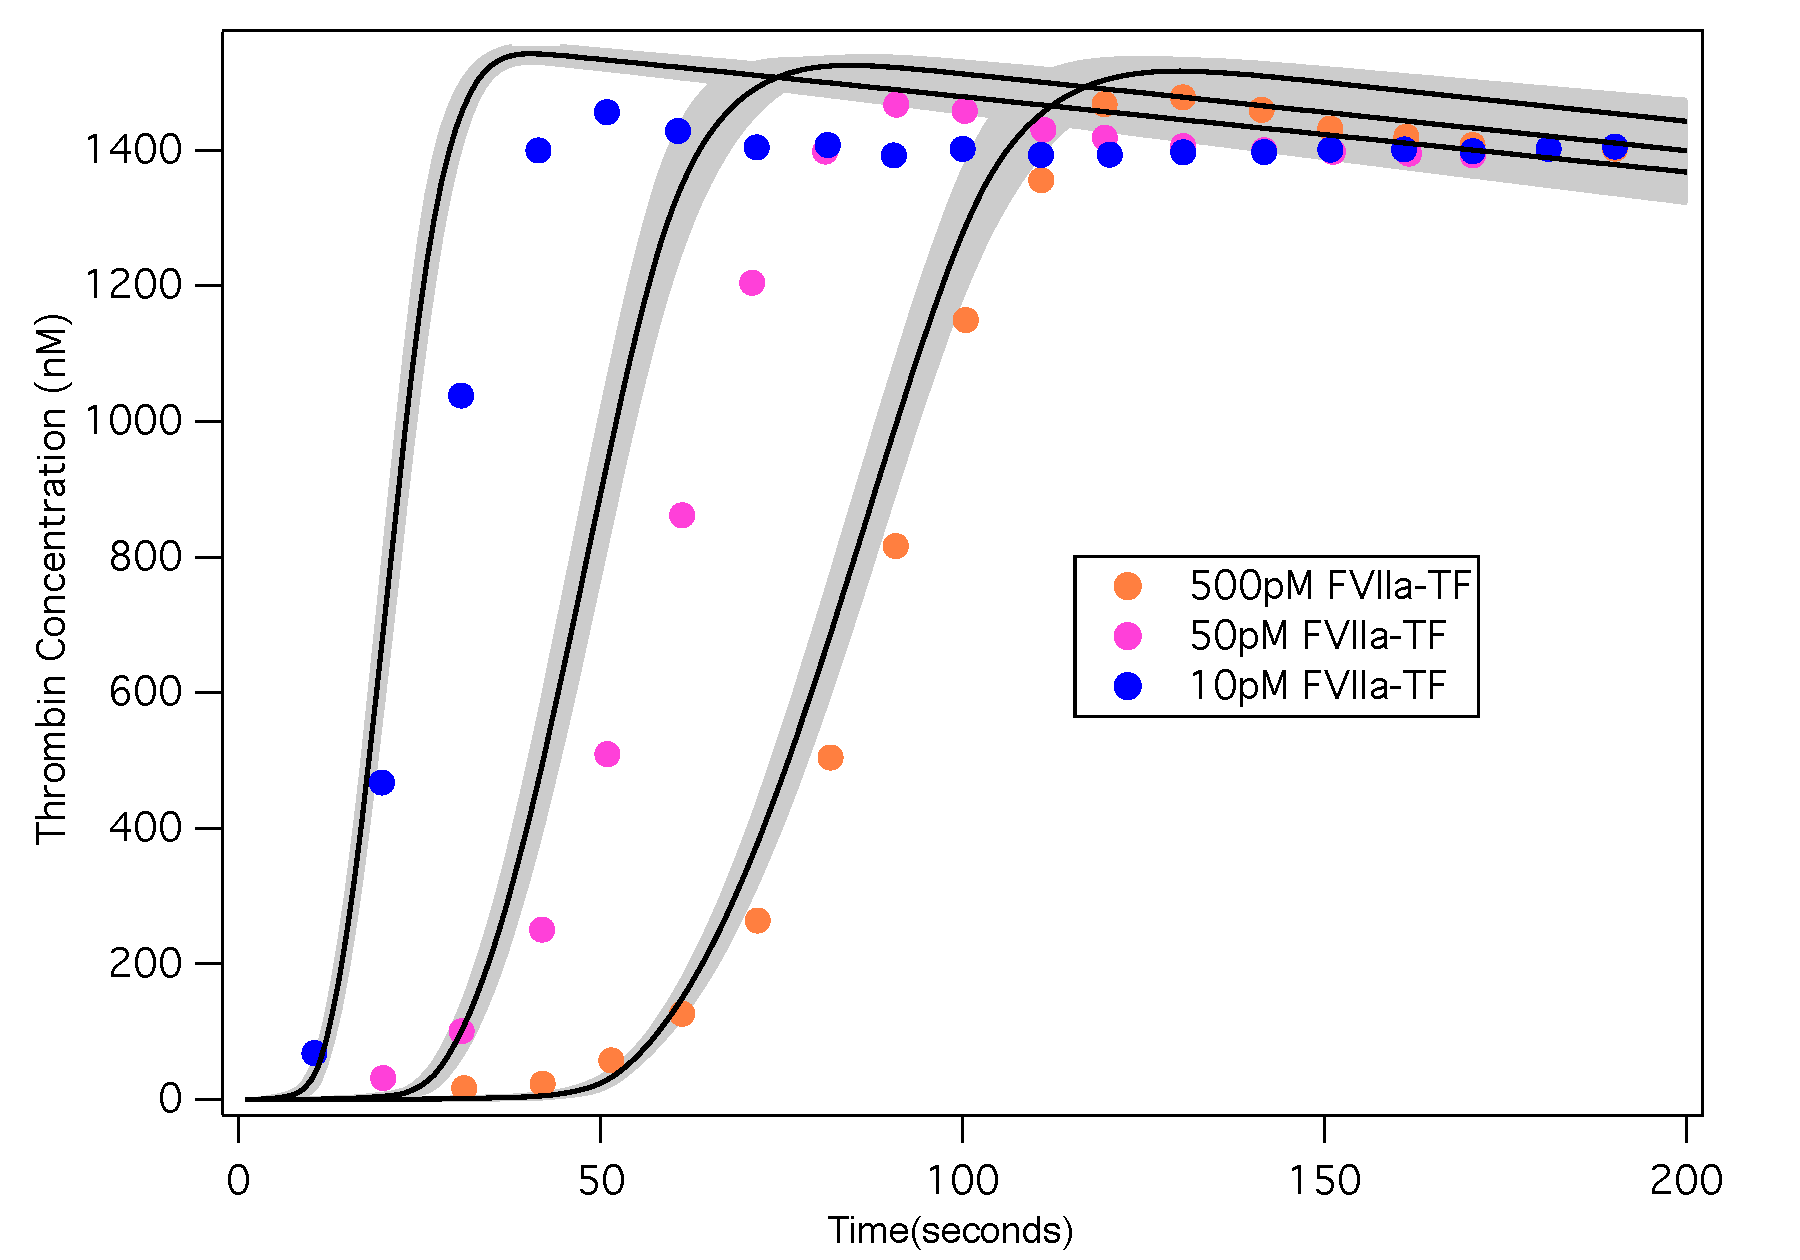
\includegraphics[width=1.0\textwidth,height=0.5\textheight]{./figs/Figure_5_Sim_Validate_E2_E4_E6.pdf}
\caption{Model predictions on unseen experimental data using parameters obtained from DDSMLSPSO. 
The parameter estimates that were obtained using DDSMLSPSO were tested against data that was not used in the model training. Solid black lines indicate the simulated mean thrombin concentration using parameter vectors from $N$= 25 trials. The grey shaded region represents the 99\% confidence estimate of the mean simulated thrombin concentration. The experimental data is reproduced from the synthetic plasma assays of Mann and co-workers [REFHERE]. Thrombin generation is initiated by adding Factor VIIa-TF (500pM - Blue, 50pM - Pink and 10pM - Orange respectively) to synthetic plasma containing 200 $\mu$mol/L of phospholipid vesicles (PCPS) and a mixture of coagulation factors (II,V,VII,VIII,IX,X and XI) at their mean plasma concentrations. 
}\label{fig-validation}
\end{figure}

\begin{figure}[H]
\centering
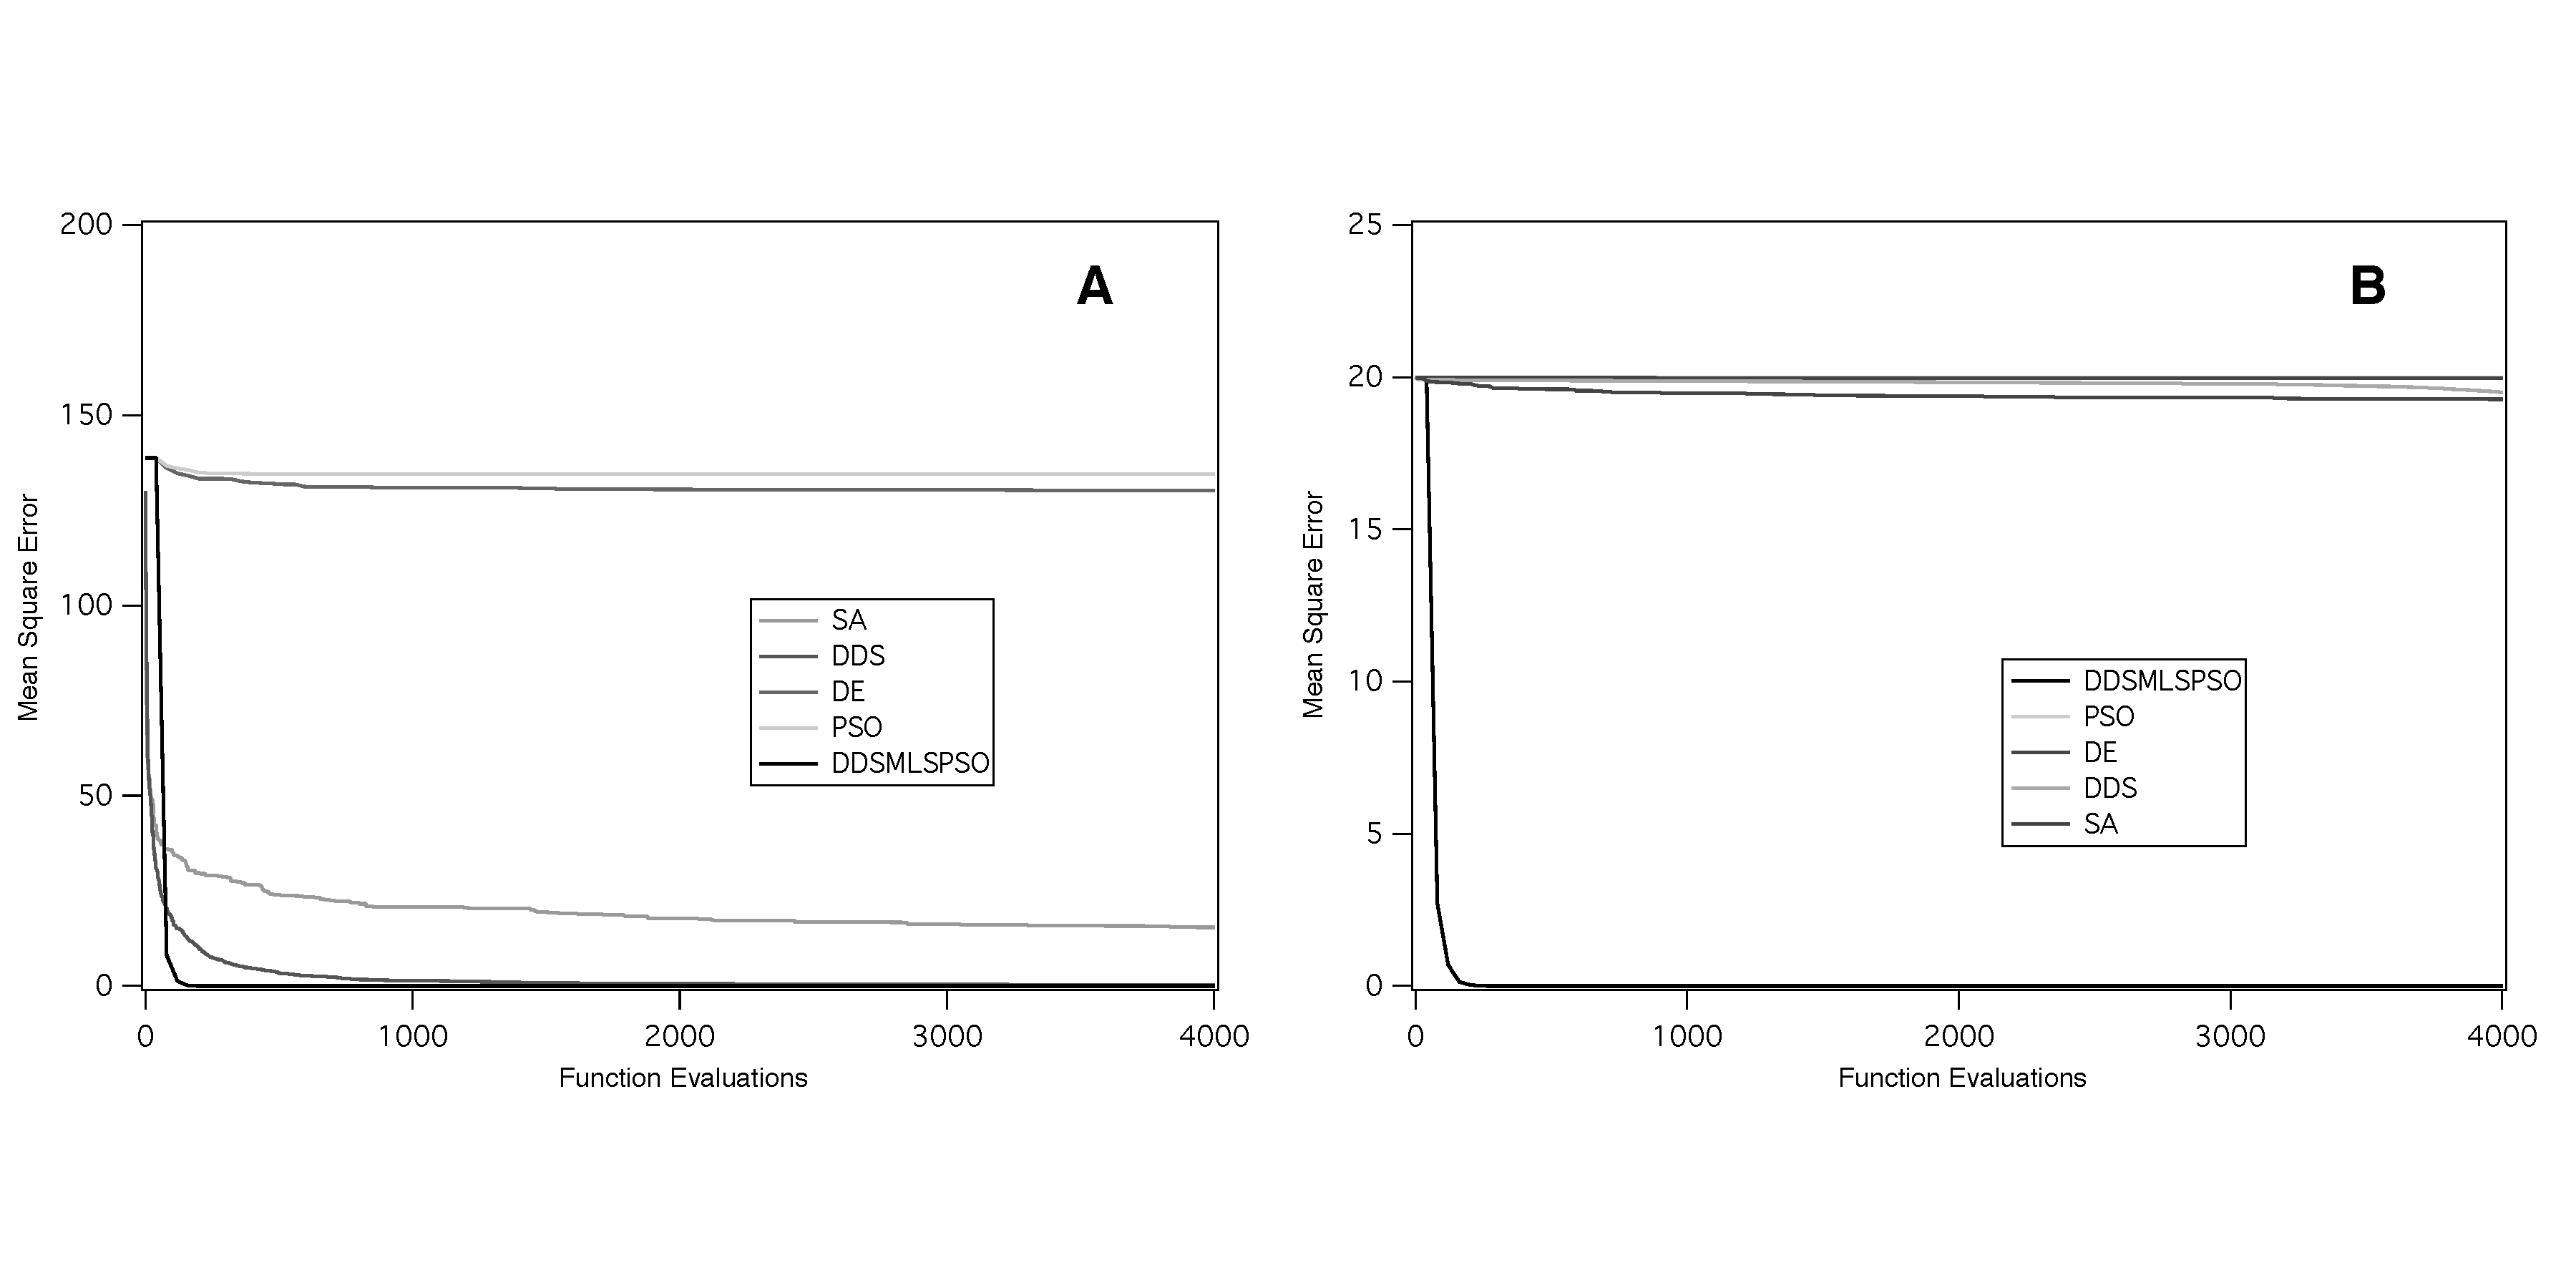
\includegraphics[width=1.02\textwidth,height=0.5\textheight]{./figs/Figure6_Ackley_Rast.pdf}
\caption{Error convergence rates on a 300 dimensional Rastrigin function and Ackley function. Ackley and Rastrigin are commonly used test functions for global optimization. DDSMLSPSO finds the minimum $ {0} $ much faster than other approaches in both cases within 4000 function evaluations \textbf {A} On a 300-D Rastrigin, DDSMLPSO, DDS and SA perform the best followed by PSO and DE  \textbf {B} On a 300-D Ackley, DDSMLSPSO clearly outperforms the rest of the algorithms.
}\label{fig-Rast}
\end{figure}


\begin{figure}[H]
\centering
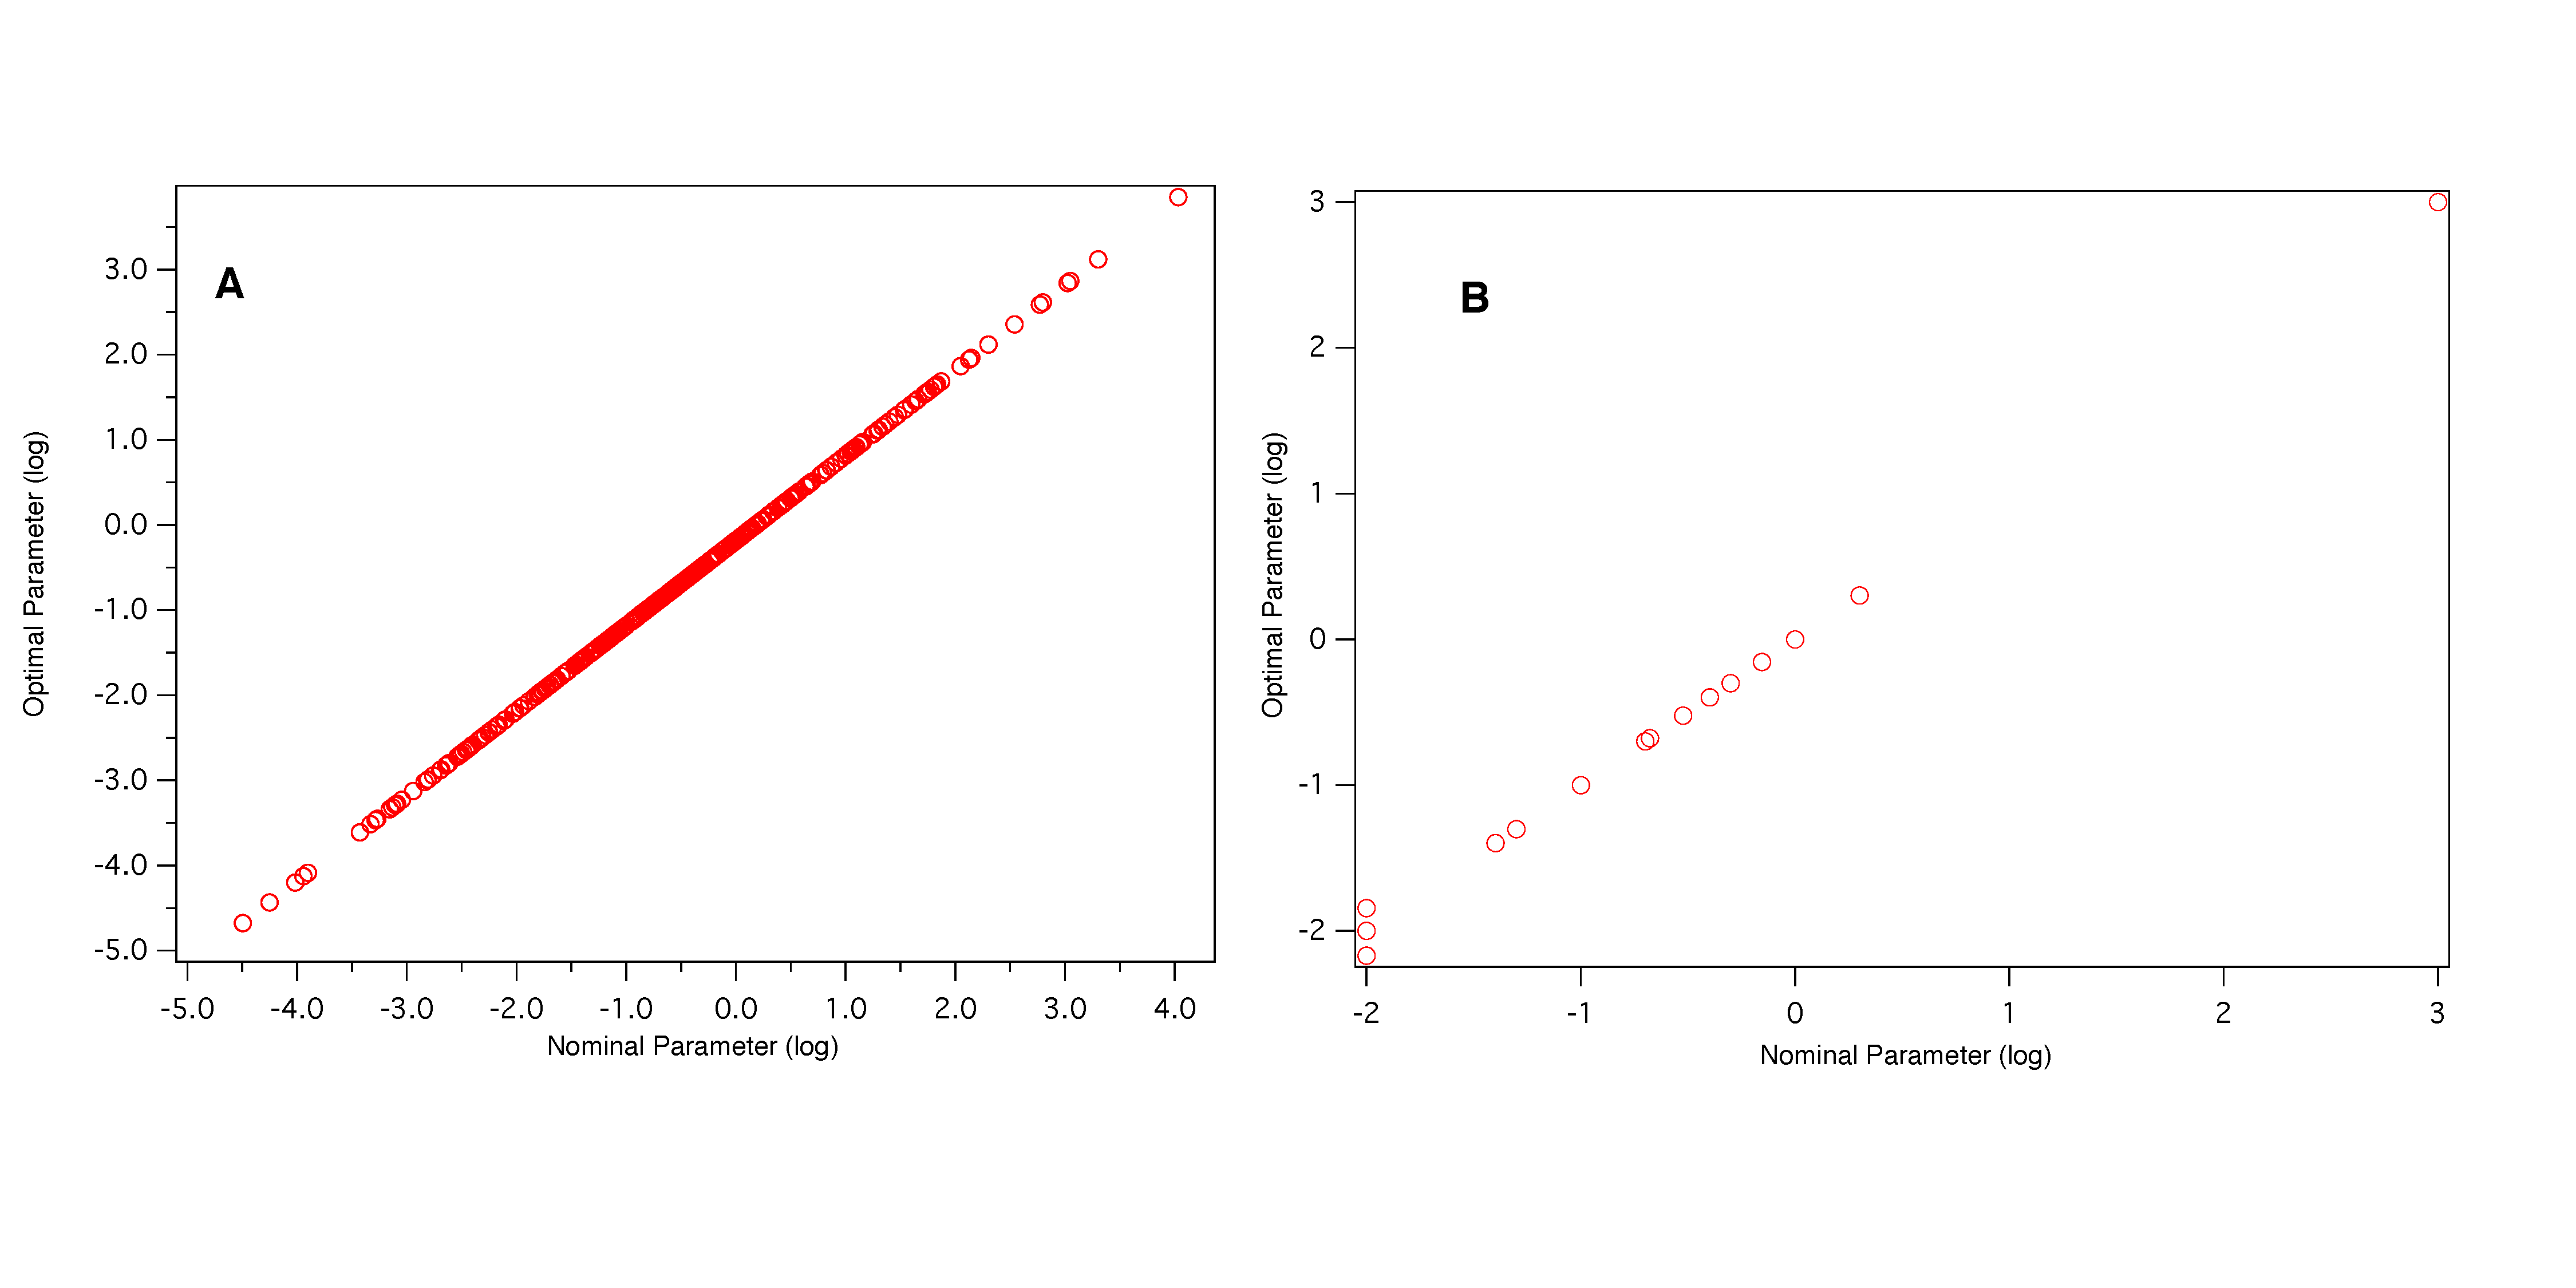
\includegraphics[width=1.02\textwidth,height=0.5\textheight]{./figs/Figure_7_Benchmarks_Parameters}
\caption{Difference between optimal and nominal parameter vector values on benchmark problems [REFHERE]. \textbf {(A)} Problem B1: Genome wide kinetic model of E.coli \textit{S.cerevisiae} with 1759 unknown parameters. \textbf {(B)} Problem B4: Metabolic model of Chinese  Hamster Ovary Cells (CHO) cells with 117 parameters.
}\label{fig-benchmark}
\end{figure}




\section*{Acknowledgements}
This study was supported by the National Science Foundation GK12 award (DGE-1045513) 
and by the National Science Foundation CAREER award (FILLMEIN).

\clearpage

\bibliography{References_v1}

%\begin{comment}

\clearpage

% Supplemental figures -
% Set the S- 
\renewcommand\thefigure{S\arabic{figure}}
\renewcommand\thetable{T\arabic{table}}
\renewcommand\thepage{S-\arabic{page}}
\renewcommand\theequation{S\arabic{equation}}

% Reset the counters -
\setcounter{equation}{0}
\setcounter{table}{0}
\setcounter{figure}{0}
\setcounter{page}{1}

\end{document}

